\documentclass[a4paper,titlepage,12pt]{article}
\usepackage[utf8]{inputenc} %Make sure all UTF8 characters work in the document
\usepackage{listings} %Add code sections
\usepackage{color}
\usepackage{graphicx}
\usepackage{titling}
\usepackage{textcomp}
\usepackage[hyphens]{url}
\usepackage[bottom]{footmisc}
\usepackage[yyyymmdd]{datetime}
\usepackage{tikz}
\usetikzlibrary{arrows}
\definecolor{listinggray}{gray}{0.9}
\definecolor{lbcolor}{rgb}{0.9,0.9,0.9}

%Set page size
\usepackage{geometry}
\geometry{margin=3cm}
\usepackage{parskip} 

\renewcommand{\dateseparator}{-}
\renewcommand{\figurename}{Figur}

\author{Emil Segerbäck -- emise935
    \and
    Malcolm Vigren -- malvi108
    }


%%%%%%%%%%%%%%%%%%%%%%%%%%%%%%%
% Header and footer
%%%%%%%%%%%%%%%%%%%%%%%%%%%%%%%
\usepackage{fancyhdr}
\pagestyle{fancy}

\lhead{Malcolm Vigren, malvi108@student.liu.se \\
Emil Segerbäck, emise935@student.liu.se}
\rhead{19950127-0970 \\
19950619-4670}


\title{\textbf{TAOP33 -- Laborationsuppgift 6}}
\date{\today}

\begin{document}
	\maketitle
	\newpage
\section*{Beskrivning}
En kommande transport av tomma godstågsvagnar mellan fyra tågstationer, A, B, C
och D ska planeras. Tågstationerna är förbunda med räls enligt figur \ref{trackfig}.
Till en början finns 47, 19, 2 och 39 vagnar vid stationerna A, B, C, D, och
stationerna behöver 2, 65, 25 respektive 15 tomma godsvagnar. Kunderna vid
varje station betalar olika mycket för varje tomvagn, 22, 28, 26 respektive 24
kr/vagn vid stationerna A, B, C respektive D. Ej efterfrågade vagnar kostar 1,
2, 3 respektive 4 kr/vagn vid varje station. Tågen ska åka enligt en viss
tidtabell, så inga extra transportkostnader tillkommer.
\begin{figure}[h]
    \begin{centering}
    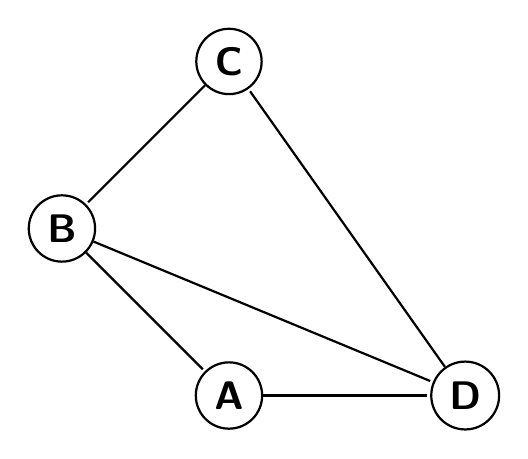
\begin{tikzpicture}[>=stealth',shorten >=1pt,auto,node distance=3cm,
                        thick,main node/.style={circle,draw,font=\sffamily\Large\bfseries}]

      \node[main node] (A) {A};
      \node[main node] (B) [above left of=A] {B};
      \node[main node] (C) [above right of=B] {C};
      \node[main node] (D) [right of=A] {D};

      \path[every node/.style={font=\sffamily\small}]
        (A) edge node {} (D)
        (B) edge node {} (A)
        (B) edge node {} (D)
        (C) edge node {} (B)
        (D) edge node {} (C);

    \end{tikzpicture}
        \caption{Modell av vägarna mellan tågstationerna\label{trackfig}}
    \end{centering}
\end{figure}

Uppgiften är planera transporten av vagnar sådan att vinsten maximeras.

\section*{Modell}
Problemet formuleras som ett maxflödesproblem. Se figur \ref{modfig} nedan.

\begin{figure}[h]
    \begin{centering}
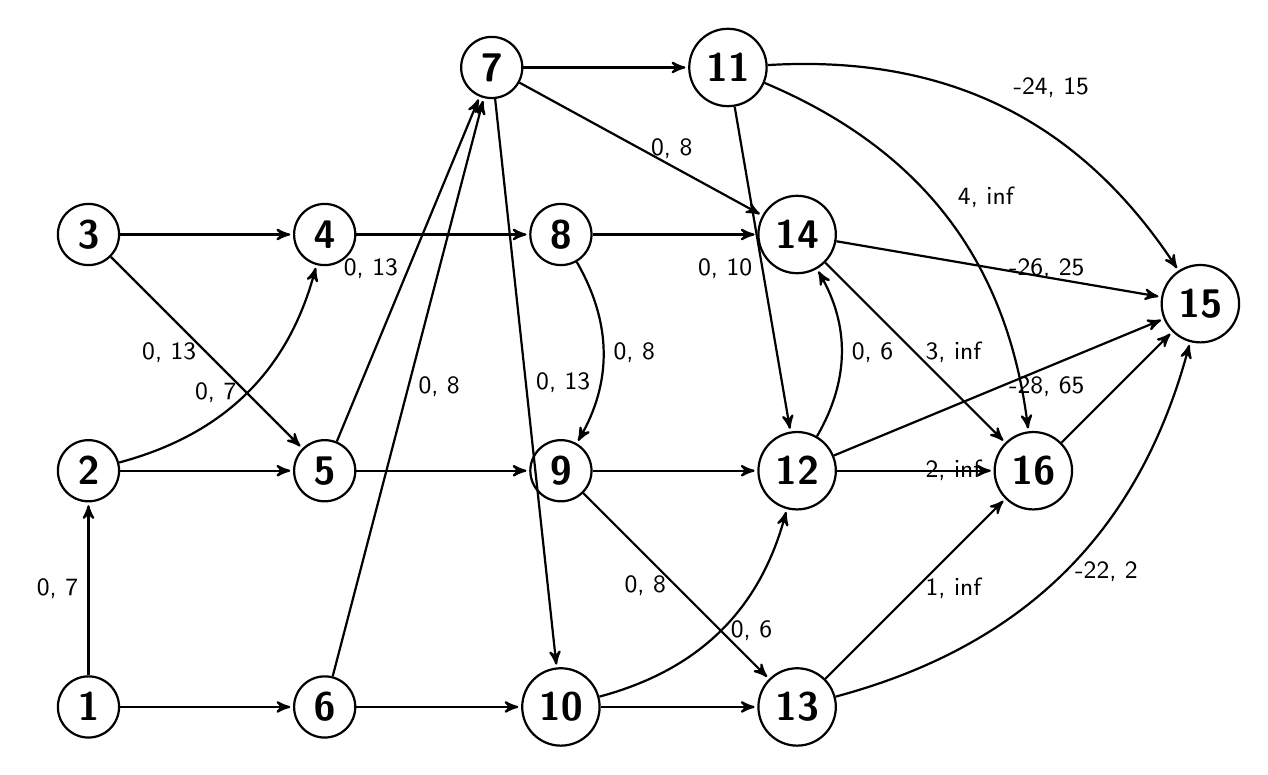
\begin{tikzpicture}[->,>=stealth',shorten >=1pt,auto,node distance=3cm,
                    thick,main node/.style={circle,draw,font=\sffamily\Large\bfseries}]

  \node[main node] (1)  [] {1};
  \node[main node] (2)  [above of=1] {2};
  \node[main node] (3)  [above of=2] {3};
  \node[main node] (4)  [right of=3] {4};
  \node[main node] (5)  [right of=2] {5};
  \node[main node] (6)  [right  of=1] {6};
  \node[main node] (7)  [above right of=4] {7};
  \node[main node] (8)  [right of=4] {8};
  \node[main node] (9)  [below of=8] {9};
  \node[main node] (10) [right of=6] {10};
  \node[main node] (11) [right of=7] {11};
  \node[main node] (12) [right of=9] {12};
  \node[main node] (13) [right of=10] {13};
  \node[main node] (14) [right of=8] {14};
  \node[main node] (16) [right of=12] {16};
  \node[main node] (15) [above right of=16] {15};

  \path[every node/.style={font=\sffamily\small}]
    (1) edge node [left] {0, 7} (2)
    (2) edge [bend right] node[left] {0, 7} (4)
    (3) edge [left] node {0, 13} (5)
    (3) edge node [left] {} (4)
    (1) edge node [left] {} (6)
    (2) edge node [left] {} (5)
    (5) edge node [left] {} (9)
    (6) edge node [left] {} (10)
    (10) edge node [left] {} (13)
    (9) edge node [left] {} (12)
    (4) edge node [left] {} (8)
    (8) edge node [left] {} (14)
    (7) edge node [left] {} (11)
    (5) edge node [left] {0, 13} (7)
    (6) edge node [right] {0, 8} (7)
    (7) edge node [right] {0, 13} (10)
    (7) edge node [right] {0, 8} (14)
    (8) edge [bend left] node[right] {0, 8} (9)
    (12) edge [bend right] node[right] {0, 6} (14)
    (11) edge [left] node {0, 10} (12)
    (9) edge node [left] {0, 8} (13)
    (10) edge [bend right] node[right] {0, 6} (12)
    (16) edge [right] node {} (15)
    (12) edge [right] node {2, inf} (16)
    (13) edge [bend right] node[right] {-22, 2} (15)
    (13) edge [right] node {1, inf} (16)
    (12) edge [right] node {-28, 65} (15)
    (14) edge [right] node {3, inf} (16)
    (14) edge [right] node {-26, 25} (15)
    (11) edge [bend left] node {4, inf} (16)
    (11) edge [bend left] node {-24, 15} (15);
\end{tikzpicture}
        \caption{Modell av problemet.\label{modfig}}
    \end{centering}
\end{figure}
Nod 1, 2, 3 och 7 representerar betraktas som källor med styrkorna 47, 19, 2
respektive 39, alltså hur många vagnar som finns på stationerna A, B, C och D.
Bågarna uppåt och nedåt representerar tåg som färdas mellan stationerna, medan
vågräta bågar representerar vagnar som lämnas kvar på stationerna. Raderna
representerar alltså stationerna, noderna 1, 6, 10 och 13 är station A, 2, 5, 9
och 12 är station B och så vidare. Bågkostnader och kapaciteter är märkta
(kostnad, kapacitet). Eftersom de vågräta bågarna är vagnar som
stannar kvar, är bågkostnader och kapaciteter inte märkta för dessa. För noder
som går upp och ner i grafen, representerar kapaciteterna hur många vagnar de
avgående tågen kan ta.

Nod 15 och 16 är speciella noder. Nod 16 representerar överblivna vagnar som
lämnats i slutet av dagen, och som man måste betala lageravgift för, vilket
representeras av bågkostnaden. Kapaciteten för bågar till nod 16 är oändliga,
då stationerna kan i teorin lagra hur många vagnar som helst. Nod 15 är en
sänka med styrka 107, som motsvarar den totala mängden vagnar som rör sig i
nätet.  Till denna nod representerar bågkostnaderna från varje station hur mycket man
tjänar per vagn (som därför blir negativa), och kapaciteten hur många vagnar
som efterfrågas. Detta gör att vagnar som inte efterfrågas måste åka till nod
16 innan de åker till 15 (en båge utan kostnad och oändlig kapacitet), 
för att betala lageravgiften.

\subsection*{Extra tågförbindelse}
Enligt problemtexten (b) kan ett extra godståg sättas in mellan station A och C,
utan att stanna vid andra stationer. Detta tåg avgår 12.30 och kommer fram
13.45 och kan ta 15 godsvagnar. Problemet blir då att hitta den högsta kostnad
som den nya förbindelsen får ha för att det ska vara lönsamt att skicka den
vägen.

I denna situation blir modellen av problemet som i figur \ref{modfig2}.

En ny länk läggs alltså till, mellan nod 6 och 8 (röd i figuren) med kapacitet
15. Den har en okänd bågkostnad \textit{a}. Problemet handlar då om att hitta
högsta värdet på \textit{a} sådan att den bågen används.

\begin{figure}[h]
    \begin{centering}
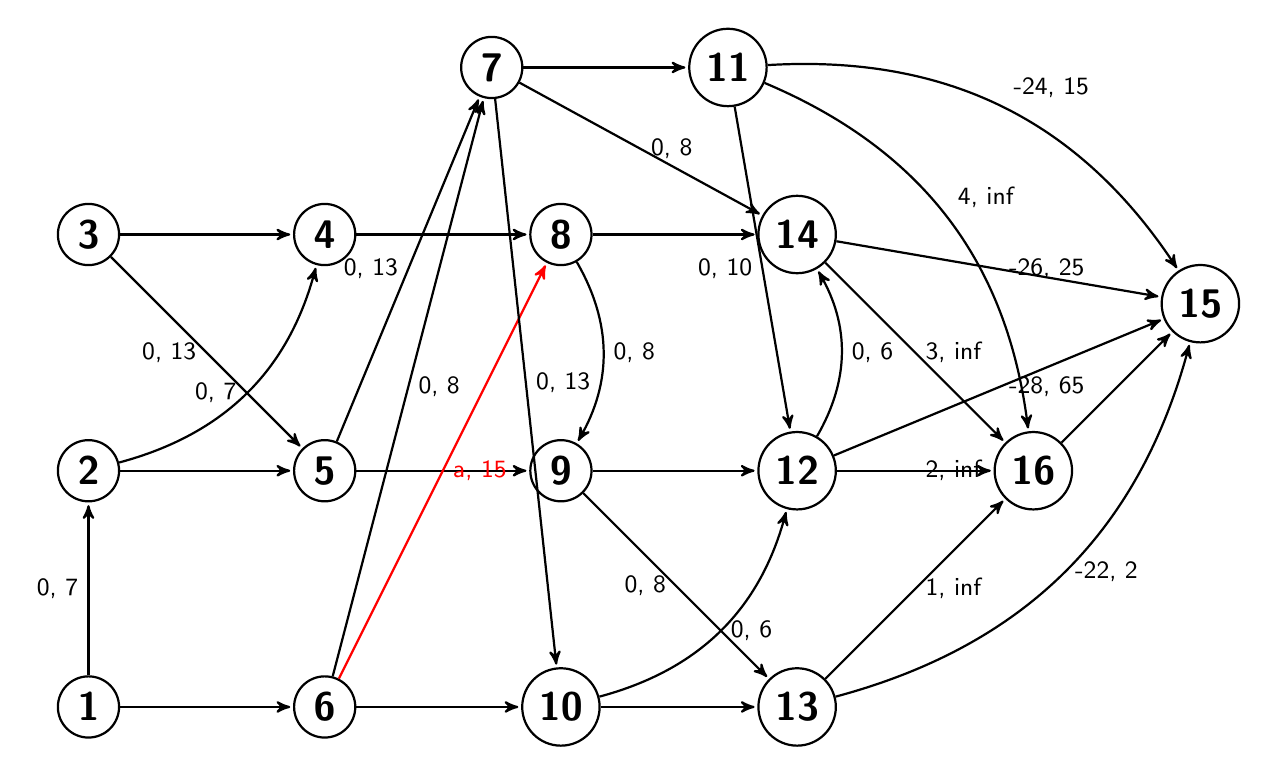
\begin{tikzpicture}[->,>=stealth',shorten >=1pt,auto,node distance=3cm,
                    thick,main node/.style={circle,draw,font=\sffamily\Large\bfseries}]

  \node[main node] (1)  [] {1};
  \node[main node] (2)  [above of=1] {2};
  \node[main node] (3)  [above of=2] {3};
  \node[main node] (4)  [right of=3] {4};
  \node[main node] (5)  [right of=2] {5};
  \node[main node] (6)  [right  of=1] {6};
  \node[main node] (7)  [above right of=4] {7};
  \node[main node] (8)  [right of=4] {8};
  \node[main node] (9)  [below of=8] {9};
  \node[main node] (10) [right of=6] {10};
  \node[main node] (11) [right of=7] {11};
  \node[main node] (12) [right of=9] {12};
  \node[main node] (13) [right of=10] {13};
  \node[main node] (14) [right of=8] {14};
  \node[main node] (16) [right of=12] {16};
  \node[main node] (15) [above right of=16] {15};

  \path[every node/.style={font=\sffamily\small}]
    (1) edge node [left] {0, 7} (2)
    (2) edge [bend right] node[left] {0, 7} (4)
    (3) edge [left] node {0, 13} (5)
    (3) edge node [left] {} (4)
    (1) edge node [left] {} (6)
    (2) edge node [left] {} (5)
    (5) edge node [left] {} (9)
    (6) edge node [left] {} (10)
    (10) edge node [left] {} (13)
    (9) edge node [left] {} (12)
    (4) edge node [left] {} (8)
    (8) edge node [left] {} (14)
    (7) edge node [left] {} (11)
    (5) edge node [left] {0, 13} (7)
    (6) edge node [right] {0, 8} (7)
    (6) edge[red] node [right] {a, 15} (8)
    (7) edge node [right] {0, 13} (10)
    (7) edge node [right] {0, 8} (14)
    (8) edge [bend left] node[right] {0, 8} (9)
    (12) edge [bend right] node[right] {0, 6} (14)
    (11) edge [left] node {0, 10} (12)
    (9) edge node [left] {0, 8} (13)
    (10) edge [bend right] node[right] {0, 6} (12)
    (16) edge [right] node {} (15)
    (12) edge [right] node {2, inf} (16)
    (13) edge [bend right] node[right] {-22, 2} (15)
    (13) edge [right] node {1, inf} (16)
    (12) edge [right] node {-28, 65} (15)
    (14) edge [right] node {3, inf} (16)
    (14) edge [right] node {-26, 25} (15)
    (11) edge [bend left] node {4, inf} (16)
    (11) edge [bend left] node {-24, 15} (15);
\end{tikzpicture}
        \caption{Modell av problemet med extra tågförbindelse\label{modfig2}}
    \end{centering}
\end{figure}

\newpage
\section*{Resultat}
Efter inmatning i VINEOPT erhålls ett flöde som i figur \ref{resfig}, i vilket
de röda siffrorna representerar flödet i de röda bågarna. Totalkostnaden för
konfigurationen blev -1806 kr, alltså en vinst på 1806 kr.

\begin{figure}[h]
    \begin{centering}
        \includegraphics[width=15cm]{res.png}
        \caption{Resultatet i VINEOPT\label{resfig}}
    \end{centering}
\end{figure}

Följande tabell beskriver vad som ska göras vid alla tågresor:

\begin{tabular}{l l l l} 
    \textbf{Tåg} & \textbf{Resa} & \textbf{Tid} & \textbf{Antal vagnar att
    medta}  \\
    1 & A-B & 09.20-10.40 & 7 \\
    1 & B-C & 10.55-12.00 & 2 \\
    2 & A-B & 16.30-17.50 & 6 \\
    2 & B-C & 18.15-19.30 & 0 \\
    3 & C-B & 11.00-12.10 & 2 \\
    3 & B-D & 12.40-14.00 & 0 \\
    3 & D-A & 14.30-15.30 & 6 \\
    4 & C-B & 15.10-16.30 & 0 \\
    4 & B-A & 16.45-17.53 & 0 \\
    5 & A-D & 13.20-14.20 & 0 \\
    5 & D-C & 14.55-16.30 & 8 \\
    6 & D-B & 16.55-17.40 & 10 \\
\end{tabular}

Detta gör att 40 vagnar lämnas på station A, 44 i B, 8 i C samt 15 i D. Man
behöver betala lagerkostnad för 38 av de vagnar som lämnats i A.

\subsection*{Extra tågförbindelse}
Prövning av olika värden visade att värdet på \textit{a} måste vara högst 28
kr/vagn. Lösningen i VINEOPT visas i figur \ref{resfig2}.

\subsection*{Skicka vagnar med persontåg}
I uppgiftstexten i (c) efterfrågades det hur mycket godsavdelningen kan betala
för att det ska vara lönsamt att skicka en vagn med ett persontåg som går från
A till C kl 16.00-17.15, samt ett vid 9.30-10.45.

Detta härleddes ur nodpriserna från modellen med extra tågförbindelse.
Nodpris för nod 14 var 27, och priset för nod 3 var 29. Därför kan vi
konstatera att man behöver betala mindre än 27 kr för tåget mellan
16.00-17.15, och mindre än 29 kr för tåget mellan 9.30-10.45, för att det ska
vara lönsamt.

\begin{figure}[h]
    \begin{centering}
        \includegraphics[width=15cm]{res2.png}
        \caption{Resultatet i VINEOPT med den extra tågförbindelsen\label{resfig2}}
    \end{centering}
\end{figure}

\newpage
\section*{Svar}

a) Maxvinst 1806

b) Kostnaden måste vara högst 28 kr per vagn. Man ska skicka 15 vagnar
med det tåget, som lämnas till slutet av dagen. Vinsten blir då 1814 kr.

c) Om man skickar 1 vagn vid 15.00-17.15 så kan godsavdelningen betala mindre än 26
kr/vagn, och vid 9.30-10.45 mindre än 28 kr/vagn.

\end{document}

